\documentclass[../main.tex]{subfiles}

\subsection{Osztálydiagram}

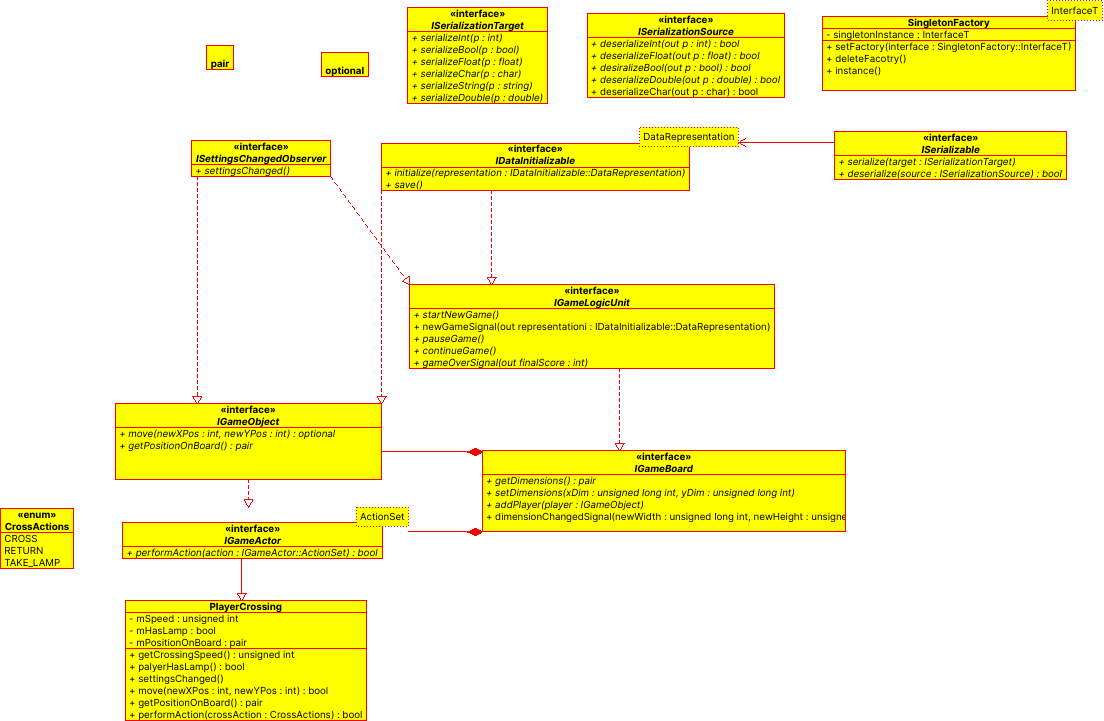
\includegraphics[width=1\textwidth]{bridge_uml.png}

\subsubsection{Vezérők, adattagok}

Az alkalmazásnak két fő logikai kompnense van, a játékos és tábla.
A tábla tartalmazza a játékost, ő hozza létre és semmisíti meg. Minden
játékosnak egyforma akciói vannak, amiket a megfelelő felsorolási típus ír le.

A nézet osztály tartalmazza a logikát és események fogagásával tájékozódik, ha a tábla a
felhasználó tevékenysége miatt változik. Tájékoztatja továbbá új játék kezdetéről, játék
végeztéről nyerés esetben. A nézet rétegnek nincs tudomása a játék éppeni folyásáról,
nem tudja ki melyik oldalon van, vagy éppen milyen stádiumban jár a kiválasztás, milyen
lépések megengedettek.

\subsubsection{Metódusok}
A játékos mozogni tud a 
\textit{MOVE\_TO\_BRIDGE}, \texit{CROSS}, \texit{RETURN} paraméterekkel,
amiket a \textbf{performAction} metódusa kap meg. Egy játékos nem léphet miden
állapotból minden állapotba, ezt a belső logikája figyeli.
A játékos általános esetben tájékozódni szeretne arról, történt-e változás a 
beállításokban. Ezt a működést az \textbf{Observer} pattern-ből ismert értesítő
\textbf{settingsChanged} metódus látja el.

A tábla a külső szemlélő számára vezérlőként működik, mert lehet elindítani,
megállítani, folytatni a rajta levő játékot, valamint lehet ezen kersztül
játékosokat mozgatni (vagy legalábbis próbálni). Ezeket a funkciókat rendre a
\textbf{startNewGame}, \textbf{pauseGame}, \textbf{continueGame} valamint \textbf{movePlayer}
metódusok látják el.

\subsubsection{Eseménykezelés}

Eseménykezelés megvalósul a nézet-tábla valamint a tábla-játékos aktorok között.
A nézet által kezelt nyomógombok a tábla bizonyos metódushívásait idézik elő.
Ezeket a hívásokat a tábla továbbítja a játékosoknak, majd eseményben tájékoztatást
kap annak sikerességéről. Természetesen az is lehet, hogy a játékos által észlelt
lépés engedélyezett, de a jelenlegi játékállapot ezt nem teszi lehetővé (például a kezdeti
oldali játékosválasztás közben az érkező oldalról akarunk játékost választani).
Ahhoz hogy a nézet nyomógombjai ne zavarják össze a játéklogikát, ezeket egy
állapotgép kezeli.

\begin{center}
\begin{tabular}{| c | c | c | c |}
    \hline
    \rowcolor{TableHeaderBlue}
    sender & signal & reciever & slot \\
    \hline
    BridgeCrossingPlayer & actionPerformedSignal & BridgeCrossingBoard & onPlayerActionPerformed \\
    \hline
    BridgeCrossingBoard & newGameSignal & BridgeCrossingViewManager & onNewGameStarted \\
    \hline
    BridgeCrossingBoard & boardChangedSignal & BridgeCrossingViewManager & onBoardChanged \\
    \hline
    BridgeCrossingBoard & scoredPointChangedSignal & BridgeCrossingViewManager & onScoredPointChanged \\
    \hline
    BridgeCrossingboard & gameOverSignal & BridgeCrossingViewManager & onGameOver \\
    \hline

\end{tabular}
\end{center}

